\chapter{直线形}

在第一章里,我们从日常生活所熟悉的位置、通路、方
向、叠合出发,讨论了空间的几个重要的基本概念:点、直
线、平行、全等、相似,并通过观察、实验,分析归纳出了
空间的一些性质。在第二章中,我们把其中的某些性质作为
基本性质和定理。在本章中,我们将以这些基本性质和定理
为基础,运用第二章所介绍的演绎法去推演空间的其它性
质。演绎法不但是研究几何学的基本有效方法,在其它任何
科学的研究中也都是十分重要的方法。概括地说,对于科学
研究,实验归纳和论证推演是互相配合使用的两种基本科学
方法,它们是探索科学规律的两条腿。从这一章起,我们对
空间性质的探讨,主要用演绎法来进行。
\section{三角形}

\subsection{全等三角形}

\begin{blk}{定义}
    平面上顺次首尾端点相接且不在同一条直线上的
线段组成的封闭图形叫做\textbf{多边形}。这些线段叫做\textbf{多边形的边},
它们的端点叫做\textbf{多边形的顶点},每相邻两边的夹角叫做多边
形的\textbf{内角}。
\end{blk}


三角形是多边形中最简单的图形。有四条边的多边形叫
做四边形,有五条边的多边形叫五边形……等等。表示一个
多边形可用顶点的名称,沿周界顺次列出,如图3.1中的
$\triangle ABC$,四边形$ABCD$……等等。

如果多边形都在每边所在直线的同旁,我们称这种多边
形为\textbf{凸多边形}(图3.1中的三个图形都是凸多边形,图3.2
中的图形则不是)。以后我们说多边形时,都指的是凸多边
形。
\begin{figure}[htp]
    \centering
    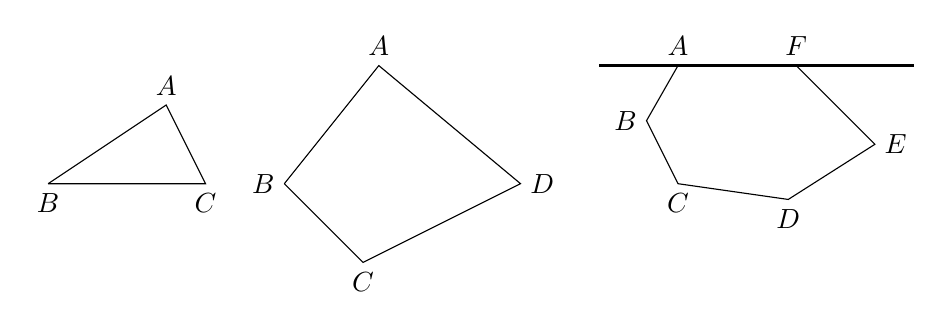
\begin{tikzpicture}
\begin{scope}
\draw(0,0)node[below]{$B$}--(2,0)node[below]{$C$}--(1.5,1)node[above]{$A$}--(0,0);
\end{scope}
\begin{scope}[xshift=3cm]
\draw (0,0)node[left]{$B$}--(1,-1)node[below]{$C$}--(3,0)node[right]{$D$}--(1.2,1.5)node[above]{$A$}--(0,0);
\end{scope}
\begin{scope}[xshift=8cm, yshift=1.5cm]
\draw (0,0)node[above]{$A$}--(1.5,0)node[above]{$F$}--(2.5,-1)node[right]{$E$}--(1.4,-1.7)node[below]{$D$}--(0,-1.5)node[below]{$C$}--(-.4,-.7)node[left]{$B$}--(0,0);
\draw[thick](-1,0)--(3,0);
\end{scope}        
    \end{tikzpicture}
    \caption{}
\end{figure}

\begin{figure}[htp]
    \centering
\begin{tikzpicture}
\draw[dashed](-2,0)--(2,0);
\draw (-.5,0)--(0.2,0)--(.3,-1)--(.7,1.8)--(-.5,0);
\end{tikzpicture}
    \caption{}
\end{figure}

\begin{blk}{定义}
两个能够完全叠合的三角形叫做\textbf{全等三角形}。两
个全等三角形完全叠合时,互相叠合的顶点叫做\textbf{对应点},互
相叠合的边叫做\textbf{对应边},互相叠合的角叫做\textbf{对应角}。因此,
\textbf{全等三角形的对应边相等,对应角相等}。
\end{blk}
 
怎样判定两个三角形全等呢?
\begin{enumerate}
\item 有两边和它们的夹角对应相等的两个三角形全
等。(SAS)
\item 有两角和它们的夹边对应相等的两个三角形全
等。(ASA)
\item 有三边对应相等的两个三角形全等。(SSS)
\end{enumerate}

利用三角形的全等,是判断两条线段或两个角相等的一
种基本方法。

\begin{example}
    在图3.3中,已知$\overline{AB}=\overline{AC}$, $\angle B=\angle C$
    
    求证:$\overline{BD}=\overline{CE}$.
\end{example}



\begin{analyze}
    要证$\overline{BD}=\overline{CE}$, 从图
上看$\overline{BD}$, $\overline{CE}$分别是$\triangle ABD$和
$\triangle ACE$的边,因此只要证明
$\triangle ACE \cong \triangle ABD$就行了,由已
知条件$\overline{AC}=\overline{AB}$, $\angle B=\angle C$而
$\angle A$是公共角,所以$\triangle ABD$与
$\triangle ACE$全等是很显然的。
\end{analyze}

\begin{proof}
在$\triangle ABD$与$\triangle ACE$中,

$\because\quad \overline{AB}=\overline{AC},\quad \angle B=\angle C$(已知)。

而$\angle A=\angle A$(公共角),

$\therefore\quad \triangle ABD\cong \triangle ACE$ (ASA).

$\therefore\quad \overline{BD}=\overline{CE}$ (全等三角形的对应边相等)。
\end{proof}    


\begin{figure}[htp]\centering
    \begin{minipage}[t]{0.48\textwidth}
    \centering
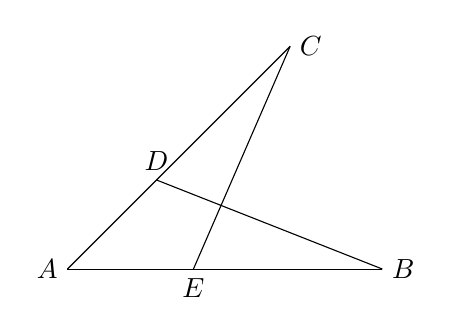
\begin{tikzpicture}[>=latex, scale=.8]
       \draw (0,0)node[left]{$A$}--(5,0)node[right]{$B$};
\draw (0,0)--(45:5)node[right]{$C$};
\draw (2,0)node[below]{$E$}--(45:5);
\draw (45:2)node[above]{$D$}--(5,0);
    \end{tikzpicture}
    \caption{}
    \end{minipage}
    \begin{minipage}[t]{0.48\textwidth}
    \centering
    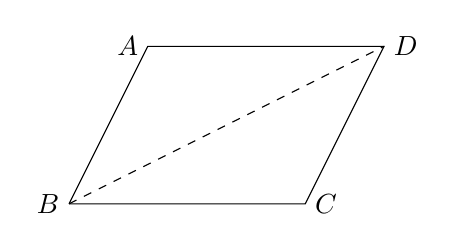
\begin{tikzpicture}[>=latex, scale=1]
        \draw (0,0)node[left]{$B$}--(3,0)node[right]{$C$}--(4,2)node[right]{$D$}--(1,2)node[left]{$A$}--(0,0);
        \draw[dashed](0,0)--(4,2);   
    \end{tikzpicture}
    \caption{}
    \end{minipage}
    \end{figure}


\begin{example}
    已知:在四边形$ABCD$中,$\overline{AD}=\overline{BC}$,
$\overline{AB}=\overline{CD}$(图3.4)。

求证:$\angle A=\angle C$。
\end{example}

\begin{analyze}
    要证明$\angle A=\angle C$, 
需要把四边形$ABCD$分成两个三
角形,为此,连结$B$、$D$. 这叫
做添\textbf{辅助线}。这样只需证
$\triangle ABD\cong \triangle CDB$就行了。
\end{analyze}

\begin{proof}
连结$B$、$D$, 在$\triangle ABD$与$\triangle CDB$中,

$\because\quad \overline{AD}=\overline{BC},\quad \overline{AB}=\overline{CD}$ (已知)

又$\because\quad \overline{BD}=\overline{BD}$ (公共边)

$\therefore\quad \triangle ABD\cong \triangle CDB$ (SSS)

$\therefore\quad \angle A=\angle C$(全等三角形的对应角相等)。
\end{proof}    

\begin{example}
在图3.5中,已知:$\overline{AB}=\overline{CD}$, $\angle B=\angle CDF$, $\overline{BD}=\overline{EF}$.

求证:$\overline{AE}=\overline{CF}$.
\end{example}

\begin{analyze}
    要证$\overline{AE}=\overline{CF}$, 只需证$\triangle ABE\cong \triangle CDF$. 由已
知,$\overline{AB}=\overline{CD}$, $\angle B=\angle CDF$, $\overline{BD}=\overline{EF}$, 虽然不能马上说
$\triangle ABE$和$\triangle CDF$全等,但只要注意到$\overline{BD}+\overline{DE}=\overline{DE}+\overline{EF}$, 
即$\overline{EB}=\overline{DF}$就行了。
\end{analyze}

\begin{proof}
    在图3-5中,$\because\quad \overline{BD}=\overline{EF}$ 已知

$\therefore\quad \overline{BD}+\overline{DE}=\overline{DE}+\overline{EF}$ (等量加等量和相等)。即:
\[\overline{BE}=\overline{DF}\]
又$\because\quad \overline{AB}=\overline{CD},\; \angle B =\angle CDF$ 已知

$\therefore\quad \triangle ABE\cong \triangle CDF$ (SAS).

$\therefore\quad \overline{AE}=\overline{CF}$ (全等三角形的对应边相等)。
\end{proof}

\begin{figure}[htp]\centering
    \begin{minipage}[t]{0.48\textwidth}
    \centering
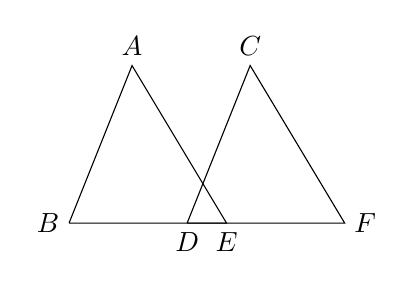
\begin{tikzpicture}[>=latex, scale=1]
       \draw(0,0)node[left]{$B$}--(2,0)node[below]{$E$}--(.8,2)node[above]{$A$}--(0,0);
\draw(1.5,0)node[below]{$D$}--(3.5,0)node[right]{$F$}--(2.3,2)node[above]{$C$}--(1.5,0);
    \end{tikzpicture}
    \caption{ }
    \end{minipage}
    \begin{minipage}[t]{0.48\textwidth}
    \centering
    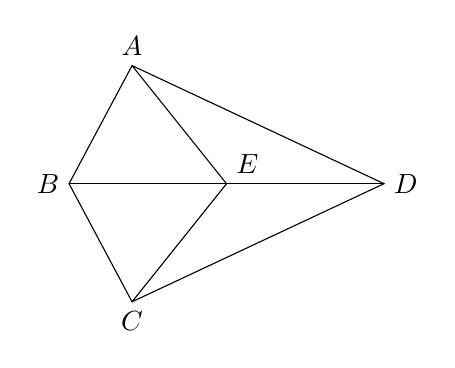
\begin{tikzpicture}[>=latex, xscale=.8]
      \draw(0,0)node[left]{$B$}--(5,0)node[right]{$D$};
      \draw(1,1.5)node[above]{$A$}--(2.5,0)node[above right]{$E$}--(1,-1.5)node[below]{$C$}--(0,0)--(1,1.5)--(5,0)--(1,-1.5);
    \end{tikzpicture}
    \caption{ }
    \end{minipage}
    \end{figure}

\begin{example}
    在图3.6中,已知:$\overline{AB}=\overline{BC}$, $\overline{AD}=\overline{CD}$, $E$点在$BD$上。

求证:$\overline{AE}=\overline{CE}$.
\end{example}

\begin{analyze}
    要证$\overline{AE}=\overline{CE}$, 只需证明$\triangle ABE\cong \triangle CBE$, 或者证明$\triangle ADE\cong \triangle CDE$, 假定我们证明$\triangle ABE\cong \triangle CBE$,
    已知$\overline{AB}=\overline{BC}$, $\overline{BE}=\overline{BE}$, 因此只需证明$\angle ABD=\angle CBD$;
    要证$\angle ABD=\angle CBD$, 只需证明$\triangle ABD\cong\triangle CBD$.
\end{analyze}

\begin{proof}
    在$\triangle ABD$与$\triangle CBD$中,

    $\because\quad \overline{AB}=\overline{CB},\quad \overline{AD}=\overline{CD}$ (已知)   $\overline{BD}=\overline{BD}$(公共边)

    $\therefore\quad \triangle ABD\cong \triangle CBD$ (SSS).

    $\therefore\quad \angle ABD=\angle CBD$ (全等三角形的对应角相等)

$\because\quad     \overline{AB}=\overline{BC}$ (已知) 
    $\overline{BE}=\overline{BE}$ (公共边)

$\therefore\quad \triangle ABE\cong \triangle CBE$ (SAS).

$\therefore\quad \overline{AE}=\overline{CE}$ (全等三角形的对应边相等)。
\end{proof}

    利用三角形全等,来证明两条线段或两个角相等,关键
    在于找出能够全等的三角形,并且使要证明的线段和角恰好
    成为它们的对应边和对应角。为了找出全等的三角形,必要
    时需要添加辅助线。  

\begin{ex}
\begin{enumerate}
    \item 已知:在四边形$ABCD$中,$AC$平分$\angle BAD$, $\overline{AB}=\overline{AD}$.
    
    求证:$\angle ACB=\angle ACD$.
    \item 已知:如图,$\overline{AC}$、$\overline{BD}$交于$O$点,    且$\overline{AO}=\overline{OC}$、$\overline{BO}=\overline{OD}$.
    
    求证:$\overline{AB}=\overline{CD}$.


\item 已知:如图,$\angle 1=\angle 4$, $\angle 2=\angle 3$.
求证:$\overline{AB}=\overline{CD}$.
\item 已知:如图,$\angle 1=\angle 2$, $\angle 3=\angle 4$, $\overline{AB}=\overline{AD}$. 

求证:$\overline{AE}=\overline{AC}$, $\angle E=\angle C$.

\item 已知:如图,$\angle 1=\angle 2$, $\angle 3=\angle 4$,
求证:$\overline{AC}=\overline{BD}$.
\item 已知:如图,在四边形$ABCD$中,$\overline{AB}=\overline{BC}$, $\overline{AD}=\overline{CD}$.

求证:$\angle A=\angle C$.
\item 已知:如图,$\overline{AD}=\overline{BE}$, $\overline{AE}=\overline{BD}$, AC、BC是直线。

求证:$\angle CDB=\angle CEA$.
\item 已知:如图,$\overline{AB}=\overline{CD}$, E、F分别是$\overline{AB}$、$\overline{CD}$的中点,
并且$\overline{BF}=\overline{CE}$.

求证:$\angle EBC=\angle FCB$, $\angle FBC=\angle ECB$.

\item 已知:如图,在四边形$ABCD$中,$\overline{AB}=\overline{CD}$, $\overline{AD}=\overline{BC}$, $\overline{EF}$过$\overline{BD}$的中点$O$. 

求证:$\overline{OE}=\overline{OF}$.
\end{enumerate}
\end{ex}

\begin{figure}[htp]\centering
    \begin{minipage}[t]{0.48\textwidth}
    \centering
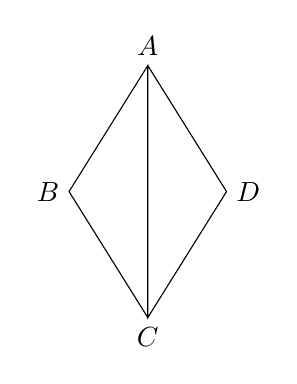
\begin{tikzpicture}[>=latex, yscale=.8]
       \draw(0,2)node[above]{$A$}--(1,0)node[right]{$D$}--(0,-2)node[below]{$C$}--(0,2)--(-1,0)node[left]{$B$}--(0,-2);
    \end{tikzpicture}
    \caption*{第1题}
    \end{minipage}
    \begin{minipage}[t]{0.48\textwidth}
    \centering
    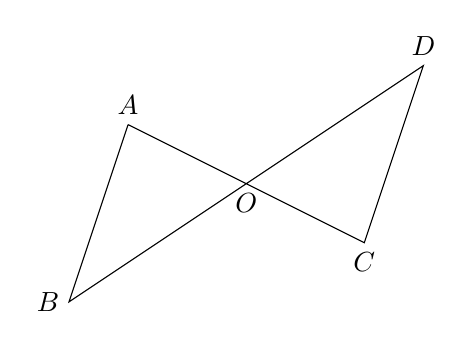
\begin{tikzpicture}[>=latex, scale=1.5]
      \draw(-1,.5)node[above]{$A$}--(1,-.5)node[below]{$C$}--(1.5,1)node[above]{$D$}--(-1.5,-1)node[left]{$B$}--(-1,.5);
      \node at (0,0)[below]{$O$};
    \end{tikzpicture}
    \caption*{第2题}
    \end{minipage}
    \end{figure}

\begin{figure}[htp]\centering
    \begin{minipage}[t]{0.48\textwidth}
    \centering
\begin{tikzpicture}[>=latex, scale=1.3]
\tkzDefPoints{1/2/A, 0/0/B, 3/0/C, 4/2/D}
\tkzDrawPolygon(A,B,C)
\tkzDrawPolygon(A,D,C)
\tkzMarkAngle[mark=none, size=.35](B,A,C)  
\tkzLabelAngle[pos=.5](B,A,C) {2}
\tkzMarkAngle[mark=none, size=.5](C,A,D)  
\tkzLabelAngle[pos=.7](C,A,D) {1}
 \tkzLabelAngle[pos=.75](A,C,B) {4}
\tkzMarkAngle[mark=none, size=.5](D,C,A)  
\tkzLabelAngle[pos=.25](D,C,A) {3}
\tkzMarkAngle[mark=none, size=.6](A,C,B) 
\tkzLabelPoints[left](A,B)
\tkzLabelPoints[right](C,D)
    \end{tikzpicture}
    \caption*{第3题}
    \end{minipage}
    \begin{minipage}[t]{0.48\textwidth}
    \centering
    \begin{tikzpicture}[>=latex, scale=1.3]
        \tkzDefPoint(0,0){A}
        \tkzDefPoint(-90:2){B}
        \tkzDefPoint(-60:2){D}
        \tkzDefPoint(0:2.75){E}
        \tkzDefPoint(-30:2.75){C}
        \tkzLabelPoints[left](A,B)
        \tkzDrawPolygon(A,B,D)
\tkzDrawLines[add=0 and 1.38](B,D) %\tkzGetPoint{C}
\draw (D)--(E)--(A)--(C);
\tkzLabelPoints[right](C,E)
\tkzLabelPoints[below](D)
\tkzMarkAngles[mark=none, size=.44](C,A,E B,A,D C,B,A E,D,A)  
\tkzLabelAngle[pos=.65](C,A,E) {2}
\tkzLabelAngle[pos=.65](B,A,D) {1}
\tkzLabelAngle[pos=.6](C,B,A) {3}
\tkzLabelAngle[pos=.6](E,D,A) {4}


    \end{tikzpicture}
    \caption*{第4题}
    \end{minipage}
    \end{figure}



\begin{figure}[htp]\centering
    \begin{minipage}[t]{0.48\textwidth}
    \centering
\begin{tikzpicture}[>=latex, scale=1]
\tkzDefPoints{-1/2/A, 1/2/D, -2/-1/B, 2/-1/C}
\tkzDrawPolygon(A,C,D) \tkzDrawPolygon(A,B,D)
\tkzLabelPoints[left](A,B)
\tkzLabelPoints[right](C,D)
\tkzMarkAngles[mark=none, size=.6](C,A,D A,D,B) 
\tkzMarkAngles[mark=none, size=.5](B,A,C B,D,C) 
\tkzLabelAngle[pos=.7](C,A,D) {1}
\tkzLabelAngle[pos=.7](A,D,B) {2}
\tkzLabelAngle[pos=.65](B,A,C) {3}
\tkzLabelAngle[pos=.65](B,D,C) {4}



    \end{tikzpicture}
    \caption*{第5题}
    \end{minipage}
    \begin{minipage}[t]{0.48\textwidth}
    \centering
    \begin{tikzpicture}[>=latex, scale=1.3]
        \tkzDefPoints{-1/0/B, 2/0/D, 1/1/A, 1/-1/C, 0/0/O} 
        \tkzDrawPolygon(A,B,C,D)
        \tkzAutoLabelPoints[center=O](A,B,C,D)

    \end{tikzpicture}
    \caption*{第6题}
    \end{minipage}
    \end{figure}




\begin{figure}[htp]\centering
    \begin{minipage}[t]{0.48\textwidth}
    \centering
\begin{tikzpicture}[>=latex, scale=1]
    \tkzDefPoints{-1.5/0/A, 1.5/0/B, 0/3/C, 0/1.5/O}  
    \tkzDefMidPoint(A,C)\tkzGetPoint{D}
    \tkzDefMidPoint(B,C)\tkzGetPoint{E}    
    \tkzDrawPolygon(A,B,C)
    \draw(B)--(D)node[left]{$D$};
    \draw (A)--(E)node[right]{$E$};
    \tkzAutoLabelPoints[center=O](A,B,C)
    \end{tikzpicture}
    \caption*{第7题}
    \end{minipage}
    \begin{minipage}[t]{0.48\textwidth}
    \centering
    \begin{tikzpicture}[>=latex, scale=.8]
        \tkzDefPoints{-2.5/0/B, 2.5/0/C, -1.5/3/A, 1.5/3/D,  0/1.5/O}  
        \tkzDefMidPoint(A,B)\tkzGetPoint{E}
        \tkzDefMidPoint(D,C)\tkzGetPoint{F}    
        \tkzDrawPolygon(A,B,C,D)
        \draw(B)--(F)node[right]{$F$};
        \draw (C)--(E)node[left]{$E$};
        \tkzAutoLabelPoints[center=O](A,B,C,D)
    \end{tikzpicture}
    \caption*{第8题}
    \end{minipage}
    \end{figure}


\begin{figure}[htp]\centering
    \begin{minipage}[t]{0.48\textwidth}
    \centering
\begin{tikzpicture}[>=latex, scale=.8]
    \tkzDefPoints{-2.5/0/B, 2.5/0/C, -1.5/3/A, 3.5/3/D}  
    \tkzDefMidPoint(D,B)\tkzGetPoint{O}
    \tkzDrawPolygon(A,B,C,D)
\draw (0,3)node[above]{$E$}--(1,0)node[below]{$F$};
\tkzAutoLabelPoints[center=O](A,B,C,D)
\draw(B)--(D);
\node at (O)[right]{$O$};

    \end{tikzpicture}
    \caption*{第9题}
    \end{minipage}
    \begin{minipage}[t]{0.48\textwidth}
    \centering
    \begin{tikzpicture}[>=latex, scale=1]
\tkzDefPoints{-1.5/0/B, 1.5/0/C, 0/3/A, 0/1.5/O}
\tkzDrawPolygon(A,B,C)
\tkzAutoLabelPoints[center=O](A,B,C)
\tkzMarkAngles[mark=none, size=.5](C,B,A A,C,B B,A,C) 
\node at (0,-.25){底};\node at (0,2.25){顶角};
\node at (-1,1.5){腰};\node at (1,1.5){腰};
\node(A) at (0,.25){底角};
\draw[<-](-1,.25)--(A);
\draw[<-](1,.25)--(A);
    \end{tikzpicture}
    \caption{}
    \end{minipage}
    \end{figure}

\subsection{等腰三角形}

\begin{blk}{定义}
    有两条边相等的三角形叫做\textbf{等腰三角形}。相等的两边
叫做\textbf{腰},另外的一边叫做\textbf{底},腰和底的夹角叫做\textbf{底角},两腰的夹
角叫\textbf{顶角},如图3.7所示。
\end{blk}

\begin{blk}{定义}
    三角形的一个角的平分线与对边相交,这个角的
    顶点和交点之间的线段叫做\textbf{三角形的角的平分线}。在图
    3.8(1)中,$\overline{AF}$平分$\angle A$, 交对边于$F$点,$\overline{AF}$就是$\triangle ABC$
    的$\angle A$的平分线。  

    连结三角形一个顶点和它的对边中点的线段叫做\textbf{三角形
的中线}。在图3.8(2)中,$E$点是$\overline{BC}$的中点,$\overline{AF}$就是$\triangle ABC$的$\overline{BC}$边上的中线。

从三角形一个顶点到它的对边所在直线作垂线,顶点和
垂足之间的线段叫做\textbf{三角形的高线}(简称\textbf{高})。在图3.8(3)
中,$\overline{AD}\bot$直线$BC$, $D$是垂足,$\overline{AD}$就是$\triangle ABC$的$\overline{BC}$边上
的高线。
\end{blk}

\begin{figure}[htp]
    \centering
\begin{tikzpicture}[scale=.8]
\begin{scope}
\tkzDefPoints{0/0/B, 3.6/0/F, 5.5/0/C, 4.5/3/A}
\tkzDrawPolygon(A,B,C)
\draw(A)--(F);
\tkzMarkAngles[mark=none, size=.5](B,A,F) 
\tkzMarkAngles[mark=none, size=.6](F,A,C)
\tkzLabelAngle[pos=.7](B,A,F) {1}
\tkzLabelAngle[pos=.75](F,A,C) {2}

\tkzLabelPoints[below](C, F, B)
\tkzLabelPoint(A){$A$}
\node at (2.7,-1){(1)};
\end{scope}
\begin{scope}[xshift=7cm]
    \tkzDefPoints{0/0/B, 2/0/E, 4/0/C, 4.5/3/A}
    \tkzDrawPolygon(A,B,C)
    \tkzLabelPoints[below](C, E, B)
    \tkzLabelPoint(A){$A$}
    \draw(E)--(A);
    \node at (2.2,-1){(2)};
\end{scope}    
\begin{scope}[yshift=-5cm]
\draw (0,0)node[below]{$B$}--(5.5,0)node[below]{$C$}--(4.5,3)node[above]{$A$}--(0,0);
\tkzDefPoints{4.5/3/A1, 4.5/0/D1, 5.5/0/C1}
\tkzMarkRightAngle(A1,D1,C1)
\draw(4.5,3)--(4.5,0)node[below]{$D$};
\draw(11,3)--(11,0)node[below]{$D$};
\draw[dashed](9,0)--(12,0);
\draw (7,0)node[below]{$B$}--(9.5,0)node[below]{$C$}--(11,3)node[above]{$A$}--(7,0);
\tkzDefPoints{11/3/A2, 11/0/D2, 9.5/0/C2}
\tkzMarkRightAngle(A2,D2,C2)
\node at (6,-1){(3)};
\end{scope}
\end{tikzpicture}
    \caption{}
\end{figure}

三角形的高线、中线、角平分线,一般是指一条线段,
但有时当我们不考虑其长度时,也把它们分别所在的直线叫
做三角形的高线、中线、角的平分线。


\begin{blk}
    {等腰三角形性质定理} 等腰三角形底角相等。
\end{blk}

已知:在$\triangle ABC$中;$AB=AC$.
求证:$\angle B=\angle C$.

\begin{figure}[htp]
    \centering
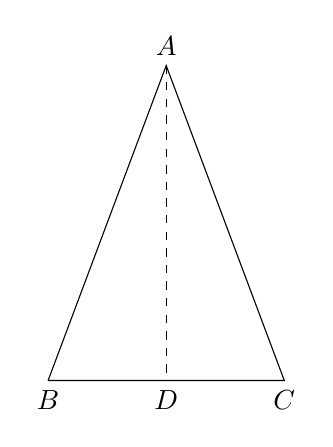
\begin{tikzpicture}
\draw (0,0)node[below]{$B$}--(3,0)node[below]{$C$}--(1.5,4)node[above]{$A$}--(0,0);
\draw[dashed](1.5,4)--(1.5,0)node[below]{$D$};
\end{tikzpicture}
    \caption{}
\end{figure}
\begin{proof}
    作$\angle BAC$的平分线$\overline{AD}$
(图3.9),在$\triangle ABD$和$\triangle ACD$
中

$\because\quad AB=AC$ (已知),$\overline{AD}=\overline{AD}$(公共边),$\angle BAD=\angle CAD$(角平分线定义)

$\therefore\quad \triangle ABD≤\triangle ACD$(SAS)

$\therefore\quad \angle B=\angle C$(全等三角形的对应角相等)。
\end{proof}


由于 $\overline{BD}=\overline{DC},\; \angle BDA=\angle CDA=90^{\circ}$

因此 $AD$平分$\overline{BC}$, 且$AD\bot BC$.

\begin{blk}{推论 }
    等腰三角形顶角的平分线垂直、平分底边。
\end{blk}

也就是说,等腰三角形的顶角平分线也是底边上的高线
和中线。(\textbf{三线合一})

\begin{blk}
    {等腰三角形的判定定理} 有两个角相等的三角形是等腰
三角形。
\end{blk}

已知:在$\triangle ABC$中,$\angle B=\angle C$(图3.10)。
求证:$\overline{AB}=\overline{AC}$.

\begin{proof}
    根据翻转公理,我们可以把$\triangle ABC$翻转过来,
    设顶点$A$、$B$、$C$成为$A'$、$B'$、$C'$.
    
    $\because\quad \angle B=\angle C=\angle C',\quad \angle C=\angle B=\angle B'$

    又:$\because\quad \overline{BC}=\overline{C'B'}$

    $\therefore\quad \triangle ABC\cong \triangle A'C'B'$(ASA)

    $\therefore\quad \overline{AB}=\overline{A'C'}$(全等三角形的对应边相等)。

由于$\overline{AC}=\overline{A'C'}$,$\therefore\quad \overline{AB}=\overline{AC}$(等量代换)
\end{proof}

用逻辑语句说:等腰三角形的判定定理是其性质定理的
逆定理。这两个定理我们用“充要”条件可合写成一个定理:

\begin{blk}{}
   一个三角形是等腰三角形的充要条件是这个三角形有两
个角相等。
\end{blk}


\begin{blk}{定义}
    三条边都相等的三角形叫做\textbf{等边三角形},也叫做
    \textbf{正三角形}。
\end{blk}


同学们自己证明下面等边三角形的性质定理和判定定
理。

\begin{blk}{}
    \begin{itemize}
        \item 等边三角形的三内角相等。
        \item   三内角相等的三角形是等边三角形。
    \end{itemize}
\end{blk}

由等腰三角形及等边三角形的性质定理和判定定理可
知,在一个三角形中,由边的相等可以推知角的相等,反过
来由角的相等也可推知边的相等。下面举例说明它们在证题
中的应用。









































